\section{Introdução}

O cenário que motivou este estudo originou-se de uma limitação operacional crítica no Ministério Público do Estado do Espírito Santo (MPES). A instituição possui um vasto acervo de atos normativos e portarias digitalizados \citep{mpes_legislacao_2026}. No entanto, o acesso a esse capital informacional era restringido pela ineficácia das ferramentas de busca disponíveis, limitadas à correspondência textual exata. Essa carência técnica tornava a recuperação da informação lenta e dependente do conhecimento tácito dos servidores sobre a estrutura dos documentos, dificultando a consulta exploratória.

Para superar essa barreira de acessibilidade e democratizar o acesso ao acervo, foi proposto o desenvolvimento de uma assistente virtual, batizada de \textbf{Fabi}, em homenagem a uma servidora reconhecida pela proficiência na navegação manual desses arquivos. Para operacionalizar a assistente e garantir que as respostas fossem fundamentadas nos documentos oficiais, mitigando o risco da geração de fatos plausíveis, porém falsos, fenômeno conhecido como alucinação \citep{ji2023}, optou-se pela arquitetura de Geração Aumentada por Recuperação (\textit{Retrieval-Augmented Generation} - RAG) \citep{lewis2020}.

A macroarquitetura da assistente Fabi integra quatro componentes fundamentais: uma interface de usuário, um motor de orquestração, um banco de dados vetorial e um modelo de linguagem gerador. O fluxo operacional do sistema, detalhado na Figura~\ref{fig:arquitetura_fabi}, segue uma lógica de processamento em etapas coordenadas.

\begin{figure}[htbp]
  \centering
  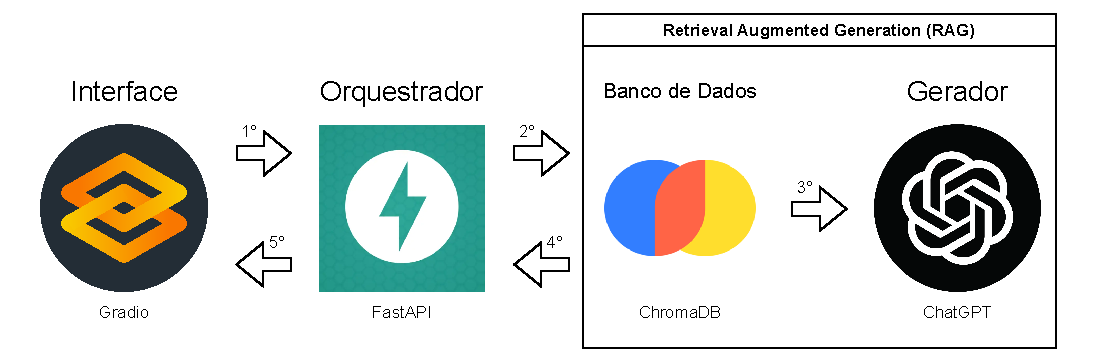
\includegraphics[width=0.8\textwidth]{figuras/arquitetura_fabi.pdf}
  \caption{Fluxo de funcionamento e componentes da arquitetura RAG da assistente Fabi.}
  \label{fig:arquitetura_fabi}
\end{figure}

O funcionamento inicia-se com a interação do usuário via interface Gradio ($1^{\circ}$), que encaminha a requisição ao orquestrador desenvolvido em FastAPI. O orquestrador envia a pergunta e a configuração de hiperparâmetros definidas ao motor RAG ($2^{\circ}$). O motor faz a recuperação de documentos relevantes e envia o contexto e a pergunta para o gerador (ChatGPT) ($3^{\circ}$). A resposta gerada é enviada de volta para o orquestrador ($4^{\circ}$), e por fim é exibida para o usuário pela interface ($5^{\circ}$)

A arquitetura RAG permite conectar a fluidez dos Grandes Modelos de Linguagem (Large Language Models - LLMs) a uma base de conhecimento externa e confiável \citep{gupta2024}. Contudo, a eficácia de um sistema RAG não é garantida apenas pela sua implementação; o desempenho é altamente sensível a hiperparâmetros de configuração, como a estratégia de segmentação dos textos (\textit{chunking}) e o volume de contexto recuperado ($k$). Configurações subótimas podem levar a respostas irrelevantes ou perda de informação crítica \citep{wang2024}.
